% =============================================================================
\bloco{2}{Growth, capital flows and national income}{Kurlat chs.~4--5; Romer chs.~1, 4 \,\textbullet\, 25 points}

\questao{(10 points) Objective items.}

\textbf{a)} (3 points) \emph{Development accounting $\times$ capital flows.} Let $Y=AK^{\alpha}(hL)^{1-\alpha}$, $\alpha\in(0,1)$, with the
same $A$ in Brazil and the US. Brazil's output per worker is a fraction $\phi$ of the US's and its human capital per worker
a fraction $\chi$, with $0<\phi<\chi<1$. The ratio of marginal products of capital (Brazil/US) implied by the
closed-economy model is:
\begin{alternativas}
\item $(1/\phi)^{(1-\alpha)/\alpha}$
\item $(\chi/\phi)^{1-\alpha}$
\item $(1/\phi)^{1-\alpha}$
\item $(\chi/\phi)^{(1-\alpha)/\alpha}$
\end{alternativas}
\gabarito{D}
\begin{sol}
\passo{MPK in observables (production function)}{Per worker $y=Ak^{\alpha}h^{1-\alpha}$, $k=K/L$, and $MPK=\partial Y/\partial K=\alpha y/k$. Inverting,
$k=\big(y/(Ah^{1-\alpha})\big)^{1/\alpha}$, so $MPK=\alpha A^{1/\alpha}(y/h)^{-(1-\alpha)/\alpha}$.}
\passo{ratio and distractors}{With common $A$, $\alpha$: $MPK_{BR}/MPK_{US}=(\chi/\phi)^{(1-\alpha)/\alpha}>1$, falling in $\alpha$ (log-derivative $-\ln(\chi/\phi)/\alpha^2$)
and tending to $1$ as $\chi\to\phi$. A sets $\chi=1$ (no human capital); B puts $y/h$ for $k/h$ in $MPK\propto(k/h)^{\alpha-1}$; C makes
both mistakes. All four exceed 1; A exceeds C and D, which exceed B, as $\chi<1$ and $(1-\alpha)/\alpha>1-\alpha$.}
\intuicao{Capital should flow to Brazil; that it does not (Lucas paradox) points to a lower $A$ (see 4(a)).}
\refbib{Kurlat (2020), \S5.3 (Lucas, 1990); Romer (2012), \S1.6, eq.~(1.32).}
\end{sol}

\medskip
\textbf{b)} (3 points) \emph{Growth $\times$ welfare.} Output per effective worker is $f(k)=A[\alpha k^{\psi}+1-\alpha]^{1/\psi}$ with $A>0$,
$\alpha\in(0,1)$, $\psi<1$, $\psi\ne0$ (elasticity of substitution $\sigma=1/(1-\psi)$), and $\dot k=sf(k)-Nk$ with $N\equiv n+g+\delta>0$.
When a Golden-Rule capital stock exists, the saving rate that attains it is:
\begin{alternativas}
\item $(\alpha A^{\psi})^{1-\psi}N^{\psi}$
\item $(\alpha A^{\psi})^{-1/(1-\psi)}N^{\psi/(1-\psi)}$
\item $(\alpha A^{\psi})^{1/(1-\psi)}N^{-\psi/(1-\psi)}$
\item $(\alpha A^{\psi})^{-(1-\psi)}N^{-\psi}$
\end{alternativas}
\gabarito{C}
\begin{sol}
\passo{Golden Rule and $f'$}{In a steady state $sf(k)=Nk$, so $c=f(k)-Nk$, strictly concave, peaks where $f'(k_{GR})=N$. As
$[\alpha k^{\psi}+1-\alpha]^{1/\psi}=f/A$: $f'(k)=\alpha A[\alpha k^{\psi}+1-\alpha]^{(1-\psi)/\psi}k^{\psi-1}=\alpha A^{\psi}(f/k)^{1-\psi}$.}
\passo{saving rate}{$f'=N$ gives $f/k=(N/\alpha A^{\psi})^{1/(1-\psi)}$; the steady state gives $s_{GR}=Nk/f$. Hence
\[s_{GR}=(\alpha A^{\psi})^{\frac1{1-\psi}}N^{-\frac{\psi}{1-\psi}}=\alpha^{\sigma}\Big(\frac AN\Big)^{\sigma-1}=\frac{k_{GR}\,f'(k_{GR})}{f(k_{GR})},\]
the capital share at $k_{GR}$, equal to $\alpha$ only in the limit $\sigma\to1$ (Cobb--Douglas).}
\passo{existence}{$f/k=A[\alpha+(1-\alpha)k^{-\psi}]^{1/\psi}$ strictly decreases, so $f'$ falls from $\infty$ to $A\alpha^{1/\psi}$ ($\psi>0$) or from $A\alpha^{1/\psi}$ to $0$
($\psi<0$): $k_{GR}$ exists iff $N>A\alpha^{1/\psi}$ ($\psi>0$) or $N<A\alpha^{1/\psi}$ ($\psi<0$), both $\iff\alpha(A/N)^{\psi}<1\iff s_{GR}<1$. Otherwise
$c$ rises without bound ($\psi>0$) or no $s<1$ sustains any $k>0$ ($\psi<0$).}
\passo{distractors}{A raises to $1-\psi$ instead of $1/(1-\psi)$ when solving $f'=N$; B inverts $sf=Nk$ (it is $1/s_{GR}$); D makes both
mistakes. As $\psi\to0$, A and C tend to $\alpha$ and B, D to $1/\alpha$: the Cobb--Douglas check cannot separate A from C.}
\intuicao{The Golden Rule reinvests capital's income; as $\partial\ln s_{GR}/\partial\ln(A/N)=\sigma-1$, only Cobb--Douglas gives ``save $\alpha$''.}
\refbib{Kurlat (2020), \S4.3; Romer (2012), \S1.4 (golden rule) and \S1.8 (elasticity of substitution).}
\end{sol}

\medskip
\textbf{c)} (2 points, T or F) Let $Y=[\alpha(BK)^{\psi}+(1-\alpha)(AL)^{\psi}]^{1/\psi}$, $\psi<1$, $\psi\ne0$, where $B$, $A$, $L$ grow at the
constant rates $g_B\ge0$, $g$, $n$. A path on which $K$ and $Y$ grow at a common constant rate exists only if $g_B=0$:
technical progress must be purely labor-augmenting.
\gabarito{T}
\begin{sol}
\passo{proof}{$(Y/K)^{\psi}=u+v$, $u\equiv\alpha B^{\psi}$, $v\equiv(1-\alpha)(AL/K)^{\psi}$; on such a path $u,v>0$ grow at constant rates $\psi g_B$, $\psi g_x$
($g_x=g+n-g_K$) and $\dot u+\dot v=\psi(g_Bu+g_xv)=0$. If $g_B\ne0$, $g_x=-g_Bu/v$ has the sign opposite to $g_B$, yet a constant $u/v$
needs $g_x=g_B$: contradiction. So $g_B=0$, then $g_x=0$: $K$ grows at $n+g$.}
\passo{the exception}{Cobb--Douglas ($\psi\to0$): $(BK)^{\alpha}(AL)^{1-\alpha}=K^{\alpha}(B^{\alpha/(1-\alpha)}AL)^{1-\alpha}$, so it binds only if $\sigma\ne1$.}
\intuicao{With $\sigma\ne1$, capital-augmenting progress moves factor shares forever.}
\refbib{Romer (2012), \S1.2 (footnote on Cobb--Douglas) and problem 1.12.}
\end{sol}

\medskip
\textbf{d)} (2 points, T or F) \emph{Growth $\times$ open economy.} In a small open Solow economy with neoclassical
$Y=F(K,AL)$, perfect capital mobility at the world rate $r^*$ and residents who save a constant fraction $s$ of national
income, a permanent rise in $s$ permanently raises GDP per worker.
\gabarito{F}
\begin{sol}
\passo{proof}{Firms rent capital until $f'(k)=r^*+\delta$, $k=K/(AL)$; $f'$ strictly decreases, so $k^*=f'^{-1}(r^*+\delta)$ is unique and free of $s$:
GDP per worker is $Af(k^*)$ at every date. Saving changes who owns capital (net foreign assets, GNI: Question~4).
The claim holds in a closed economy and for GNI per worker: that is the trap.}
\intuicao{Capital flows, not domestic saving, finance the domestic capital stock.}
\refbib{Romer (2012), problem 4.4; Kurlat (2020), \S1.1 (GDP measures production inside the country).}
\end{sol}

% -----------------------------------------------------------------------------
\questao{(15 points) Discursive. \emph{Growth $\times$ national accounts $\times$ capital flows.} Brazil as a small open
economy. Output is $Y=K^{\alpha}(AhL)^{1-\alpha}$, $\alpha\in(0,1)$; capital moves freely and earns the world rate $r^*>0$ net of
depreciation $\delta>0$; $A$ grows at $g\ge0$ and $L$ at $n\ge0$, with $n+g>0$; $h>0$ is constant. Residents own wealth $W$
(capital at home or abroad) and save a fraction $s\in(0,1)$ of gross national income (wages plus the gross return on
wealth): $\dot W=s\,\mathrm{GNI}-\delta W$. Let $N\equiv n+g+\delta$; per effective worker, $k=K/(AhL)$, $y=Y/(AhL)$, $\omega=W/(AhL)$.}

\textbf{a)} (3 points) Characterize capital and GDP per effective worker, $k^*$ and $y^*$, and their dynamics. What does a
rise in $s$ do to GDP per worker? Under perfect mobility, which ratio of labor-augmenting productivity $A_{BR}/A_{US}$ (this
question's $A$) reconciles the gaps $\phi$ and $\chi$ of Question~3(a), and what does it say about the Lucas paradox?
\resolespaco
\begin{sol}
\passo{capital is pinned (firm's FOC)}{Firms maximize $K^{\alpha}(AhL)^{1-\alpha}-(r^*+\delta)K-wL$: $\alpha k^{\alpha-1}=r^*+\delta$, whose left side falls from $\infty$
to $0$. The unique root holds at every date (capital flows in or out instantly):
\[k^*=\Big(\frac{\alpha}{r^*+\delta}\Big)^{\frac1{1-\alpha}},\qquad y^*=k^{*\alpha}=\Big(\frac{\alpha}{r^*+\delta}\Big)^{\frac{\alpha}{1-\alpha}},\qquad(r^*+\delta)k^*=\alpha y^*.\]
So GDP per worker $Ahy^*$ grows at $g$ from $t=0$ with no transition, $\partial y^*/\partial s=0$, and wages per effective worker are $(1-\alpha)y^*$.}
\passo{Lucas paradox (link to 3(a))}{The same $r^*$, $\alpha$, $\delta$ give the same $k^*$, $y^*$, so output per worker is proportional to $Ah$:
$\phi=(A_{BR}/A_{US})\chi$, i.e.\ $A_{BR}/A_{US}=\phi/\chi<1$; in the Hicks-neutral units of 3(a), $(\phi/\chi)^{1-\alpha}$, which sets its MPK ratio to $1$.}
\intuicao{Openness makes capital, not saving, adjust; small capital flows reveal a productivity gap.}
\refbib{Romer (2012), problem 4.4; Kurlat (2020), \S5.3.}
\rubrica{
\item $k^*$ from the firm's FOC, unique: 1 pt (quoted: max.\ a third of the item); $y^*$ constant, $\partial y^*/\partial s=0$: 1 pt.
\item $A_{BR}/A_{US}=\phi/\chi$ (or $(\phi/\chi)^{1-\alpha}$ in the Hicks-neutral units of 3(a)): 1 pt. Paradox read without the
link to 3(a): max.\ half of the item.
}
\end{sol}

\textbf{b)} (3 points) Derive the law of motion of wealth per effective worker, its steady state $\omega^*$ and the condition
for stability. For which world rates is wealth stable at every saving rate?
\resolespaco
\begin{sol}
\passo{national income}{Wages are $(1-\alpha)Y$ and wealth earns $r^*+\delta$ gross: $\mathrm{GNI}/(AhL)=(1-\alpha)y^*+(r^*+\delta)\omega$.}
\passo{law of motion}{$\dot\omega/\omega=\dot W/W-n-g$ ($h$ constant) and the saving rule give
\[\dot\omega=s(1-\alpha)y^*-\Lambda\,\omega,\qquad\Lambda\equiv N-s(r^*+\delta).\]}
\passo{solution and stability}{Linear: $\omega(t)=\omega^*+(\omega(0)-\omega^*)e^{-\Lambda t}$, $\omega^*=s(1-\alpha)y^*/\Lambda$, half-life $\ln2/\Lambda$; it converges iff $\Lambda>0$,
i.e.\ $s<N/(r^*+\delta)$. If $\Lambda\le0$, $\dot\omega\ge s(1-\alpha)y^*>0$ for $\omega\ge0$: wealth explodes. As $\Lambda$ falls with $s$ and is $n+g-r^*$
at $s=1$, wealth is stable at every $s\in(0,1)$ iff $r^*\le n+g$.}
\intuicao{A unit of wealth adds $s(r^*+\delta)$ through reinvested income and loses $N$ to depreciation and dilution.}
\refbib{Romer (2012), \S1.3 (same method) and \S1.5 (speed of convergence).}
\rubrica{
\item GNI per effective worker: 1 pt (return on wealth omitted: max.\ 1 pt in the item); law of motion and solution: 1 pt.
\item $\Lambda>0$ proved, case $r^*\le n+g$: 1 pt. Stability asserted without the solution: 0 for this line.
}
\end{sol}

\textbf{c)} (3 points) Assume from now on that wealth converges. Find the saving rate $\bar s$ above which Brazil is a
net creditor in the steady state and interpret it; compare it with the Golden-Rule saving rate that Question~3(b) gives for
this technology. Find GNI/GDP in the steady state in closed form.
\resolespaco
\begin{sol}
\passo{net foreign assets}{They are $\omega^*-k^*$ per effective worker. By $(r^*+\delta)k^*=\alpha y^*$ from (a), and
$s(1-\alpha)(r^*+\delta)-\alpha\Lambda=s(r^*+\delta)-\alpha N$:
\[\omega^*-k^*=\frac{s(1-\alpha)y^*}{\Lambda}-\frac{\alpha y^*}{r^*+\delta}=\frac{y^*(s-\bar s)}{\Lambda},\qquad\bar s\equiv\frac{\alpha N}{r^*+\delta}=\frac{Nk^*}{y^*}.\]
With $\Lambda>0$, Brazil is a net creditor iff $s>\bar s$.}
\passo{reading and Golden Rule}{$\bar s$ sustains $k^*$ in a closed economy ($\bar sy^*=Nk^*$); $\bar s<N/(r^*+\delta)$ as $\alpha<1$, and $\bar s<1$ iff $r^*+\delta>\alpha N$.
Cobb--Douglas gives $s_{GR}=\alpha$ (3(b), $\sigma\to1$), and $\bar s-\alpha=\alpha(n+g-r^*)/(r^*+\delta)$: if $r^*>n+g$ a Golden-Rule saver is a
creditor; at $r^*=n+g$, $\bar s=\alpha$ and $k^*=k_{GR}$ (as $f'(k^*)=N$).}
\passo{GNI/GDP}{From (b), $\mathrm{GNI}/\mathrm{GDP}=(1-\alpha)+(r^*+\delta)\omega^*/y^*=(1-\alpha)[1+s(r^*+\delta)/\Lambda]$, so
\[\frac{\mathrm{GNI}}{\mathrm{GDP}}=\frac{(1-\alpha)N}{\Lambda}=(1-\alpha)+\alpha\frac{\omega^*}{k^*},\qquad\frac{\omega^*}{k^*}=\frac{s(1-\alpha)(r^*+\delta)}{\alpha\Lambda},\]
and $\mathrm{GNI}/\mathrm{GDP}-1=(r^*+\delta)(s-\bar s)/\Lambda$: creditor status and GNI above GDP are the same statement.}
\intuicao{Net foreign assets earn the world return: GNI exceeds GDP exactly when residents own more than home capital.}
\refbib{Romer (2012), \S1.4 and problem 4.4; Kurlat (2020), \S2.1 (GNP versus GDP).}
\rubrica{
\item NFA and creditor condition, using $\Lambda>0$: 1.5 pts (threshold quoted: max.\ a third of the item).
\item Comparison with $s_{GR}$: 0.5 pt (one parameter point only: max.\ half); GNI/GDP and its link to $\bar s$: 1 pt.
}
\end{sol}

\textbf{d)} (3 points) At $t=0$ the saving rate rises once and for all from $s_0$ to $s_1$, with $s_0<\bar s<s_1$, both stable. Draw
$\dot\omega$ against $\omega$ for both rates, marking $k^*$ and the steady states. Find the date $T$ at which Brazil becomes a net
creditor, and the paths of GNI/GDP and GDP per worker.
\resolespaco
\begin{sol}
\passo{phase lines (from (b))}{$\dot\omega=s_i(1-\alpha)y^*-\Lambda_i\omega$, $\Lambda_i=N-s_i(r^*+\delta)$: intercept $s_i(1-\alpha)y^*$, slope $-\Lambda_i$, zero $\omega_i^*$. As
$\partial\dot\omega/\partial s=(1-\alpha)y^*+(r^*+\delta)\omega>0$, the $s_1$ line is above and flatter ($\Lambda_1<\Lambda_0$); by (c), $\omega_0^*<k^*<\omega_1^*$.}
\begin{center}
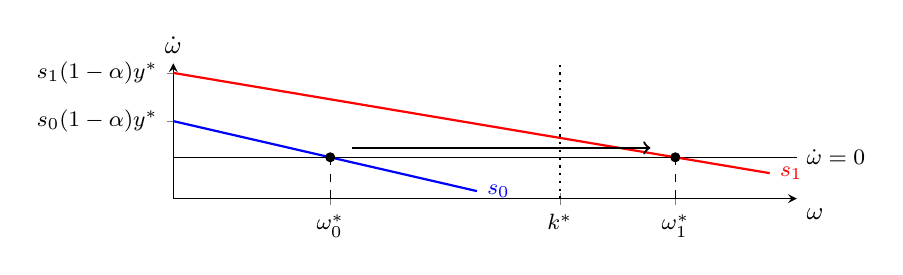
\begin{tikzpicture}
\begin{axis}[width=9.5cm,height=3.3cm,xmin=0,xmax=11.5,ymin=-0.22,ymax=0.5,axis lines=left,
  xlabel={$\omega$},ylabel={$\dot\omega$},xlabel style={at={(axis description cs:1,0)},anchor=north west},
  ylabel style={at={(axis description cs:0,1)},rotate=-90,anchor=south},
  xtick={2.894,7.128,9.259},xticklabels={$\omega_0^*$,$k^*$,$\omega_1^*$},
  ytick={0.1925,0.4490},yticklabels={$s_0(1-\alpha)y^*$,$s_1(1-\alpha)y^*$},
  tick label style={font=\footnotesize},label style={font=\small},clip=false]
\addplot[thin,domain=0:11.5]{0} node[right,font=\footnotesize]{$\dot\omega=0$};
\addplot[thick,blue,domain=0:5.6]{0.19245-0.0665*x} node[right,font=\footnotesize]{$s_0$};
\addplot[thick,red,domain=0:11]{0.44905-0.0485*x} node[right,font=\footnotesize]{$s_1$};
\addplot[dotted,thick] coordinates {(7.128,-0.22) (7.128,0.5)};
\addplot[dashed,thin] coordinates {(2.894,-0.22) (2.894,0)};
\addplot[dashed,thin] coordinates {(9.259,-0.22) (9.259,0)};
\addplot[only marks,mark=*,mark size=1.6pt] coordinates {(2.894,0) (9.259,0)};
\draw[->,thick] (axis cs:3.3,0.05) -- (axis cs:8.8,0.05);
\end{axis}
\end{tikzpicture}
\end{center}
\passo{path and crossing date}{From $\omega(0)=\omega_0^*$, $\omega(t)=\omega_1^*-(\omega_1^*-\omega_0^*)e^{-\Lambda_1t}$, increasing. $\omega(T)=k^*$ and (b)--(c), where $y^*$ cancels, give
\[T=\frac1{\Lambda_1}\ln\frac{\omega_1^*-\omega_0^*}{\omega_1^*-k^*}=\frac1{\Lambda_1}\ln\frac{(1-\alpha)N(s_1-s_0)}{\Lambda_0(s_1-\bar s)}>0,\]
as numerator minus denominator is $(\bar s-s_0)\Lambda_1>0$; $T\to0$ as $s_0\to\bar s$ and $T\to\infty$ as $s_1\downarrow\bar s$.}
\passo{GNI and GDP}{GNI/GDP $=(1-\alpha)+\alpha\,\omega(t)/k^*$ rises from $(1-\alpha)N/\Lambda_0<1$ to $(1-\alpha)N/\Lambda_1>1$, crossing $1$ at $T$; the half-life
rises to $\ln2/\Lambda_1$; GDP per worker stays on $Ahy^*$.}
\intuicao{The reform is wealth accumulation, not capital deepening: GNI moves, GDP does not.}
\refbib{Romer (2012), \S1.4 (a change in the saving rate) and problem 4.4.}
\rubrica{
\item Graph: axes, labels, intercepts, slopes, $s_1$ above and flatter: 0.5 pt; $\omega_0^*<k^*<\omega_1^*$, motion: 0.5 pt.
\item $\omega(t)$, $T$: 1 pt; $T>0$ proved: 0.5 pt (asserted: 0 for this line); GNI/GDP and GDP: 0.5 pt.
}
\end{sol}

\textbf{e)} (3 points) \emph{Parameter analysis.} How do $\omega^*/k^*$, GNI/GDP, the half-life of wealth and $\bar s$ respond to $s$, $r^*$,
$n+g$, $\delta$ and $\alpha$? Prove each sign, collect the signs in a table, give the limits as $s\to0$ and as $s$ approaches its
upper bound, and read the knife-edge cases $s=\bar s$ and $r^*=n+g$.
\resolespaco
\begin{sol}
\passo{closed forms (from (b)--(c))}{With $R\equiv r^*+\delta$, $\Lambda=N-sR>0$: $\omega^*/k^*=s(1-\alpha)R/(\alpha\Lambda)$, GNI/GDP $=(1-\alpha)+\alpha\,\omega^*/k^*=(1-\alpha)N/\Lambda$,
half-life $\ln2/\Lambda$, $\bar s=\alpha N/R$. The derivatives of $\Lambda$ in $s$, $r^*$, $n+g$, $\delta$, $\alpha$ are $-R$, $-s$, $1$, $1-s>0$, $0$.}
\passo{$s$, $r^*$, $n+g$}{The half-life moves against $\Lambda$: $+,+,-$. Except in $\alpha$, GNI/GDP moves with $\omega^*/k^*$, whose derivatives are
$(1-\alpha)NR/(\alpha\Lambda^2)>0$, $(1-\alpha)Ns/(\alpha\Lambda^2)>0$, $-(1-\alpha)sR/(\alpha\Lambda^2)<0$. For $\bar s$: $0$, $-\alpha N/R^2<0$, $\alpha/R>0$.}
\passo{$\delta$ and $\alpha$}{$\delta$ raises $N$, $R$ one for one: $\partial(R/\Lambda)/\partial\delta=(N-R)/\Lambda^2$, $\partial\bar s/\partial\delta=\alpha(R-N)/R^2$, $N-R=n+g-r^*$: $\omega^*/k^*$
and GNI/GDP move with $\operatorname{sgn}(n+g-r^*)$, $\bar s$ against it; the half-life falls. $\alpha$ enters only via $(1-\alpha)/\alpha$, $1-\alpha$,
$\alpha$: $\omega^*/k^*$ and GNI/GDP fall, $\bar s$ rises, the half-life is unchanged.}
\begin{center}
\begin{tabular}{lccccc}
\toprule
 & $s$ & $r^*$ & $n+g$ & $\delta$ & $\alpha$ \\
\midrule
$\omega^*/k^*$, GNI/GDP & $+$ & $+$ & $-$ & $\operatorname{sgn}(n+g-r^*)$ & $-$ \\
half-life & $+$ & $+$ & $-$ & $-$ & $0$ \\
$\bar s$ & $0$ & $-$ & $+$ & $\operatorname{sgn}(r^*-n-g)$ & $+$ \\
\bottomrule
\end{tabular}
\end{center}
\passo{limits and knife-edges}{$s\to0$: $\omega^*/k^*\to0$, GNI/GDP $\to1-\alpha$ (only wages), half-life $\to\ln2/N$. As $s\uparrow\min\{1,N/R\}$: if $r^*\ge n+g$,
$\Lambda\downarrow0$ and all three explode (smallness fails first); if $r^*<n+g$ they stay finite (GNI/GDP $\to(1-\alpha)N/(n+g-r^*)$). At
$s=\bar s$: $\omega^*=k^*$, GNI $=$ GDP, $\Lambda=(1-\alpha)N$, the closed-economy speed. At $r^*=n+g$: $\delta$ drops out of both
ratios and $\bar s=\alpha=s_{GR}$.}
\intuicao{Openness separates where capital works from who owns it: more return reinvested from wealth ($s$, $r^*$)
relative to dilution ($n+g$) enriches residents at unchanged output; $\alpha$ shrinks the wage bill that funds saving;
$\delta$ cuts $k^*/y^*=\alpha/R$ and raises $\Lambda$, the first more iff $r^*<n+g$.}
\refbib{Romer (2012), \S1.5 and problem 4.4; Kurlat (2020), \S1.1 (GDP) and \S2.1 (GNP).}
\rubrica{
\item $\Lambda$'s derivatives and the twenty signs, proved: 1.5 pts (a sign without proof: 0 for that entry).
\item Table, limits, knife-edges: 1 pt. Column readings: 0.5 pt (no proofs or no reading: max.\ half).
}
\end{sol}
